\chapter*{Anexo A}
\label{chap:anexoA}
{\Large \bfseries Tiempo invertido y diagrama de Gantt}

El diagrama de Gantt en la Figura~\ref{fig:diagrama_gantt} refleja las diferentes fases del proyecto y la dedicación en
el tiempo invertidos. Todo comienza con un periodo de investigación donde
se adquieren los conocimientos previos necesarios. Seguidamente, comienza la etapa de diseño e
implementación de la herramienta desarrollada. Finalmente, el periodo de elaboración de la
memoria. Por otro lado, la Tabla~\ref{tab:horas} detalla el tiempo invertido en cada una de estas fases.

\begin{figure}[htbp]
  \centering
  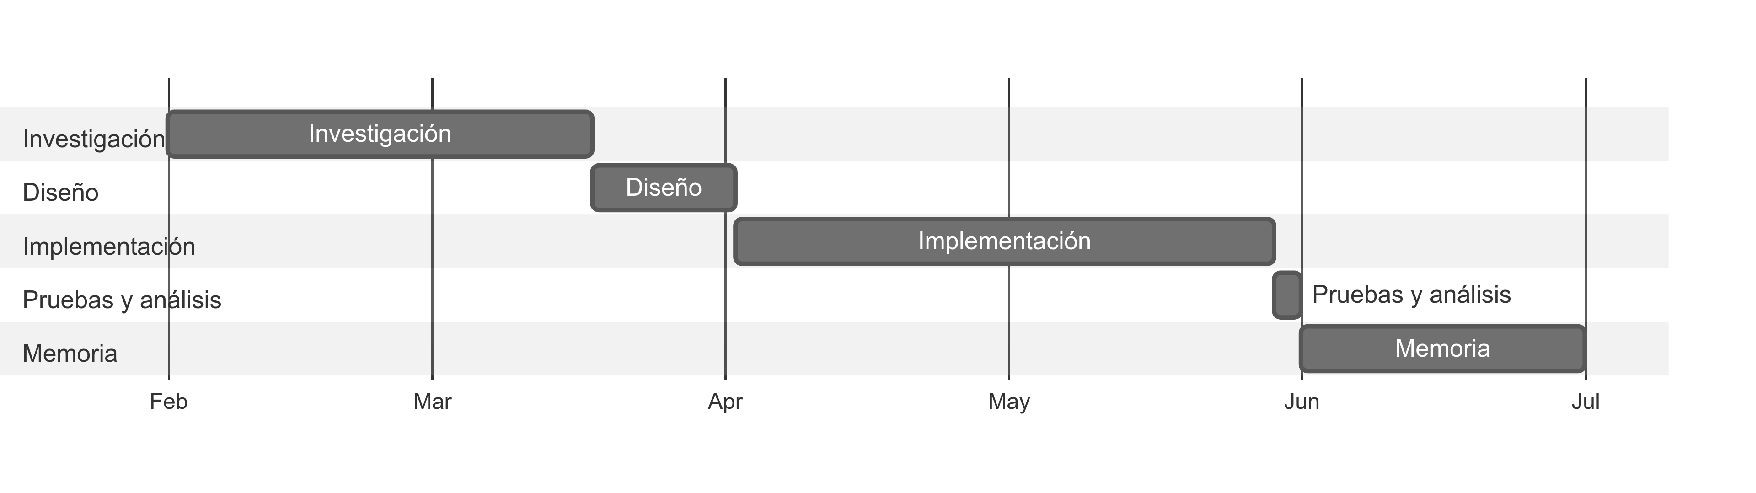
\includegraphics[width=\textwidth]{Diagrama_Gantt.pdf}
  \caption{Diagrama de gantt}
  \label{fig:diagrama_gantt}
\end{figure}

\begin{table}[H]
\centering
\small
\begin{tabular}{|l|r|}
\hline
\textbf{Fase} & \textbf{Horas} \\
\hline
\texttt{Investigación} & 25 \\
\texttt{Diseño} & 40 \\
\texttt{Implementación} & 220 \\
\texttt{Pruebas y análisis} & 20 \\
\texttt{Memoria} & 100 \\
\hline
\texttt{Total} & 405 \\
\hline
\end{tabular}
\caption{Horas invertidas}
\label{tab:horas}
\end{table}